\documentclass[11pt,a4paper]{article}

\usepackage{amsmath}
\usepackage{amsfonts}
\usepackage{amssymb}
\usepackage{graphicx}
\usepackage{enumitem}
\setlist{parsep=0pt,listparindent=\parindent}
\usepackage[left=1in,right=1in,top=1in,bottom=1in]{geometry}

\title{Machine Learning in Complex Domains:\\Assignment 2}
\author{Daniel Deutsch, Dan Crankshaw, Ryan Cotterell}
\date{}

\begin{document}

	\maketitle
	
	\setcounter{section}{2}
	\section{Problem Set}
	
	\subsection{Learning: Parameter Estimation}
	
	\setcounter{subsubsection}{4}
	\subsubsection{Analytical Questions}
	
	% 3.1.5
	\begin{enumerate}
		\item Overfitting typically occurs in a complex model when the number of
		parameters is much larger than the number of observations. When you overfit
		the data, the model is more likely to exaggerate noise in the data instead of
		lessening its effect. In this problem, consider the case if the robot reaches
		location $(i,j)$ at time $t$. If the robot does not observe a wall to the north
		when it should, the model will learn that it should never observe a wall to the north
		when at location $(i,j)$ at time $t$. We can think of this mistake the model made
		as noise. The model learned the noise to be true, so whenever the robot is at
		$(i,j)$ at time $t$, it will always predict the robot will observe no wall. This noise
		in the data has been exaggerated to always be true. 
		
		Therefore, when you are dealing with many parameters that are independent with respect
		to a specific variable, it is important to use parameter sharing so this situation 
		does not happen and you lessen the effect of noise in the data. In this assignment,
		we say that a robot observing a wall is independent of the time it happens so that
		the model does not learn parameters for each time step and learn the noise into
		the model.
		
		\item Suppose that in our model, the floor at location $(i,j)$ is very sticky. When
		the robot tries to leave this location, it is more likely not to move compared to
		other locations on he map. When we use parameter sharing, we lose the information
		about moving in direction with respect to each position, and we can no longer encode
		that information. Parameter sharing makes the assumption that the probability of moving
		in a specific direction is the same for every position, and if that assumption is not true,
		parameter sharing cannot learn this model.
		
		\item In order to combine these two approaches, you need to be able to detect an 
		anomaly within the data, like a robot not being able to move as well in a specific location
		compared to the rest. A way to do this is to compute the statistics for every location
		individually. In our problem, this would be counting the number of times the robot
		is able to move in each direction in every location. Say that the sticky location
		is at $(i,j)$. 
		
		To detect that this is an anomaly, we will iterate over all of the positions, leaving 1
		position out each time. Compute the average success of leaving the location and 
		the rest of the locations. If the probability of leaving the sticky square is significantly
		different than from the rest of the locations, then leave that location out of the 
		parameter sharing because it is an anomaly. Then you can learn parameters for 
		each of the specific anomalies and shared parameters for the rest. 
		
		With this approach, you can learn the specific parameters for each space that you
		need to and general parameters for when it does not matter. In this way, you have
		taken the advantages of both solutions.

	\end{enumerate}
	
	\subsection{Inference}
	
	\subsubsection{Analytical Questions: Clique Tree}
	
	% 3.2.1
	\begin{enumerate}
		\item The process we used to create the clique tree is drawn out graphically
		in the file {\tt CliqueTree Building.pdf}. The strategy we took was to try and do
		a small example (when the number of steps = 3), then try to generalize
		that clique tree to any arbitrary number of time steps.
		
		We made it as the instructions said: we converted the original graph into an
		undirected graph by marrying the parents of nodes at a v-structure; we converted
		the graph to a chordal graph, and verified that it was a valid chordal graph; we 
		extracted the maximal cliques from the graph and formed the cluster graph over
		these cliques; finally, we found a maximal spanning tree that we thought made
		sense intuitively and could generalize. We tried to select the MST such that there
		was a pattern in the structure that we could generalize. 
		
		When we were selecting the MST, we could have selected a different, but equally 
		valid MST that would have produced another clique tree that is different from what 
		we used. The ordering which we selected nodes in the algorithm to create a chordal
		graph was also important because if you did not select the nodes in an intelligent
		order, it was possible that the chordal graph would have been connected in a strange
		way. For example, there was a possibility that {\tt PositionRow\_t-1} would have
		been directly connected to {\tt PositionRow\_t+1}. If we allowed for that to happen,
		I believe that our resulting clique tree might be larger, more complicated, or less
		intuitive.
		
		\item We have verified that the running intersection property holds. We wrote a 
		program in {\tt test.RunningIntersectionChecker.java} that takes a list of the
		the variables and finds all of the cliques whose scope contains them. Then we
		ran a breadth-first search to find a path, only adding an edge to the queue if the
		other clique contained that same variable. If for all variables and for all of the
		cliques contain them in their scope, there exists a path from each clique
		to every other clique such that all of the cliques along that path contain the
		variable in their scope, then the running intersection property holds. Our program
		verified that our clique trees are correct.
		
		\item We made the {\tt cliquetree} file by generalizing the clique tree that we
		came up with in {\tt CliqueTree Building.pdf}. We then wrote a Python script to
		output a clique tree for an arbitrary number of time steps and landmarks, the
		only variables that change between each clique tree. The script that we wrote is
		called {\tt create-clique.py}.
	\end{enumerate}		
	
	\setcounter{subsubsection}{4}
	\subsubsection{Empirical Questions: Message Passing}
	
	% 3.2.5
	\begin{enumerate}
		\item In order to find the distribution over the final position of the robot, we added
		all of the evidence for the respective files to the model after calibration. Then we ran
		the queries
		\begin{verbatim}
		    PositionRow_t=1,PositionCol_t=1
		    PositionRow_t=1,PositionCol_t=2
		    ...
		    PositionRow_t=10,PositionCol_t=10
		\end{verbatim}
		for $t = 9, 99$ and $999$.
		
		For the {\tt network-grid10x10-t10.txt} file, our resulting probabilities were:
		\begin{center}
			\begin{tabular}{|c|cccccccccc|}
				\hline
				10 & 0.00 & 0.01 & 0.48 & 1.57 & 0.89 & 1.14 & 0.16 & 2.77 & 1.03 & 0.32 \\
				9 & 0.02 & 0.01 & 0.50 & 1.55 & 0.96 & 10.27 & 1.97 & 0.27 & 2.29 & 0.13 \\
				8 & 0.02 & 0.40 & 0.62 & 8.51 & 3.09 & 0.14 & 0.17 & 0.24 & 1.21 & 1.82 \\
				7 &0.32 & 0.28 & 0.32 & 0.19 & 0.20 & 1.81 & 0.26 & 0.61 & 0.16 & 0.09 \\
				6 & 0.01 & 0.04 & 0.01 & 0.19 & 0.28 & 1.08 & 0.10 & 0.05 & 0.02 & 0.43 \\
				5 & 0.11 & 2.50 & 0.36 & 0.04 & 0.59 & 1.88 & 0.23 & 0.02 & 0.10 & 0.31 \\
				4 & 0.77 & 2.70 & 0.04 & 0.34 & 2.71 & 1.57 & 0.11 & 0.12 & 0.05 & 0.17 \\
				3 & 0.04 & 0.03 & 0.06 & 0.18 & 0.63 & 0.34 & 2.10 & 0.01 & 0.68 & 5.55 \\
				2 & 0.08 & 0.03 & 0.02 & 0.17 & 0.25 & 3.56 & 0.74 & 2.04 & 2.04 & 2.01 \\
				1 & 0.02 & 0.00 & 0.41 & 1.78 & 4.26 & 0.54 & 3.39 & 0.33 & 4.96 & 0.10 \\
				\hline
				 & 1 & 2 & 3 & 4 & 5 & 6 & 7 & 8 & 9 & 10 \\
				 \hline
			\end{tabular}
		\end{center}
		Where the value at row $i$ and column $j$ is the percent probability of the
		robot ending up at position $(i,j)$.

		\begin{figure}[H!]
			\label{contour10}
			\begin{center}
				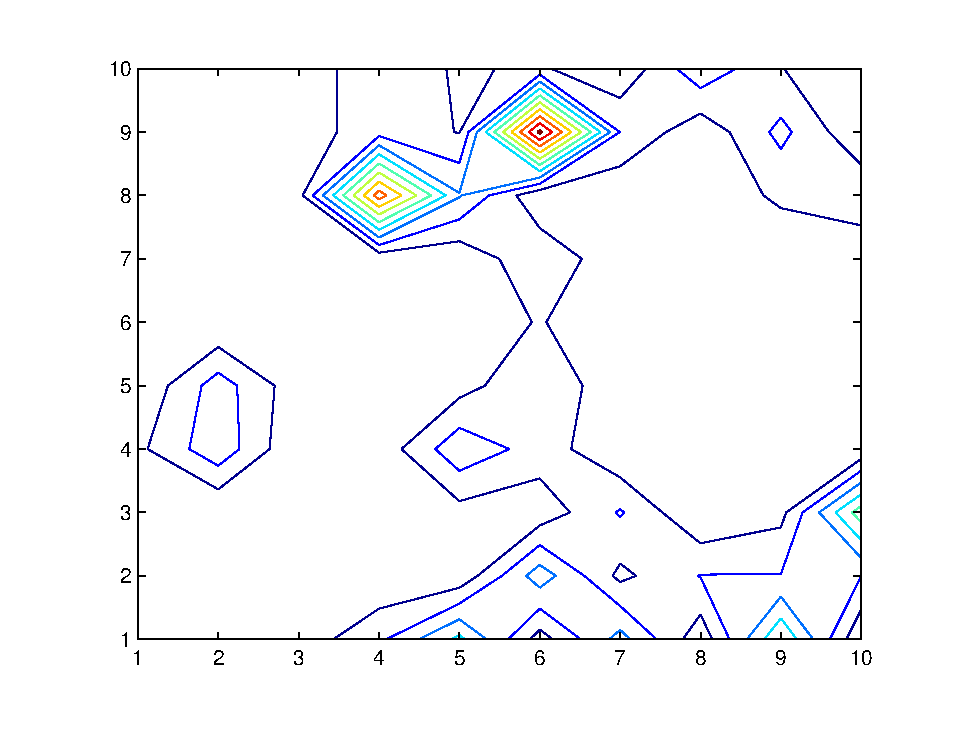
\includegraphics[scale=0.75]{t10-contour.eps}
			\end{center}
			\caption{The contour plot for t10}
		\end{figure}
		As you can see from the contour plot for t10 in Figure \ref{contour10}, the most
		likely location for the robot at time $t=9$ is the top middle of the map.
		
		For the {\tt network-grid10x10-t100.txt} file, our resulting probabilities were:
		\begin{center}
			\begin{tabular}{|c|cccccccccc|}
				\hline
				10 & 0.01 & 0.02 & 0.67 & 3.48 & 2.31 & 2.99 & 0.35 & 2.94 & 2.33 & 0.35 \\
				9 & 0.12 & 0.01 & 0.63 & 1.96 & 0.49 & 0.59 & 2.19 & 0.31 & 2.18 & 0.40 \\
				8 & 0.05 & 0.61 & 0.65 & 0.45 & 2.68 & 0.51 & 0.39 & 0.61 & 3.03 & 3.50 \\
				7 & 0.35 & 0.03 & 0.44 & 0.28 & 0.36 & 2.69 & 0.39 & 0.57 & 0.36 & 0.16 \\
				6 & 0.02 & 0.06 & 0.01 & 0.39 & 0.81 & 3.11 & 0.18 & 0.10 & 0.07 & 0.42 \\
				5 & 0.10 & 0.09 & 0.39 & 0.05 & 2.59 & 2.11 & 0.47 & 0.07 & 0.43 & 0.84 \\
				4 & 2.40 & 0.10 & 0.03 & 0.40 & 3.72 & 3.66 & 0.70 & 0.42 & 0.07 & 0.47 \\
				3 & 0.06 & 0.05 & 0.12 & 0.36 & 0.55 & 0.81 & 3.03 & 0.02 & 3.81 & 0.26 \\
				2 & 0.12 & 0.06 & 0.15 & 0.42 & 0.61 & 2.56 & 0.06 & 3.04 & 0.10 & 3.91 \\
				1 & 0.07 & 0.01 & 0.50 & 3.10 & 2.12 & 0.45 & 3.10 & 0.18 & 3.32 & 0.31 \\
				\hline
				& 1 & 2 & 3 & 4 & 5 & 6 & 7 & 8 & 9 & 10 \\
				\hline
			\end{tabular}
		\end{center}
		and the corresponding contour plot is in Figure \ref{contour100}. From the Figure,
		you can see that the robot is likely in the middle or the bottom right of the map.
		\begin{figure}[h]
			\label{contour100}
			\begin{center}
				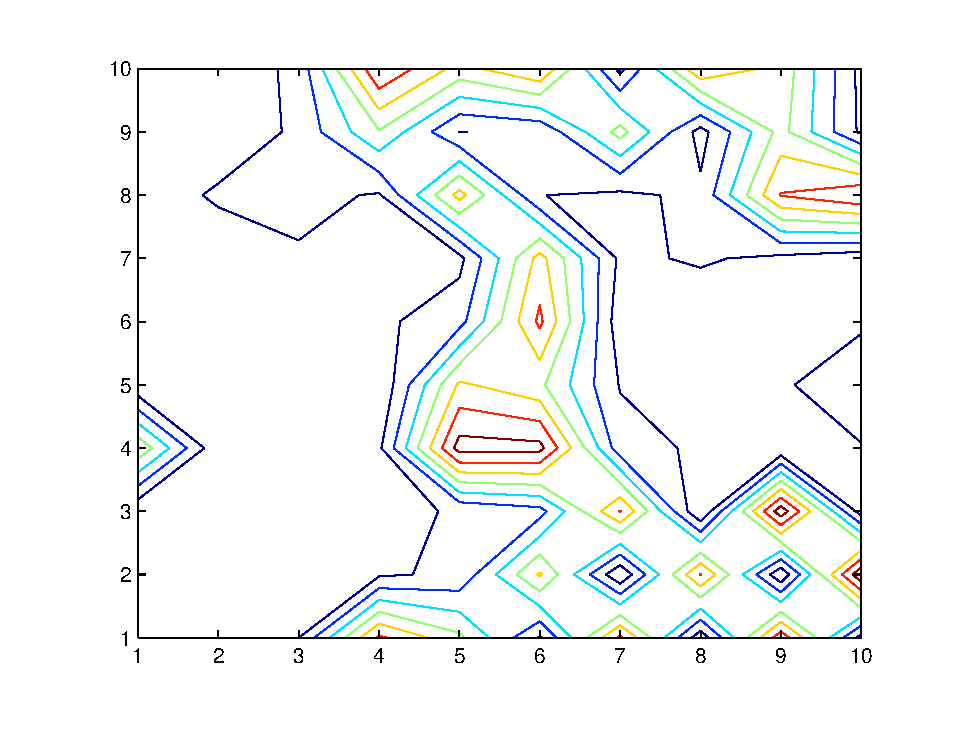
\includegraphics[scale=.75]{t100-contour.eps}
			\end{center}
			\caption{The contour plot for t100}
		\end{figure}
		
		
		\item
		\item
		\item
		\item
		\item
	\end{enumerate}
	
	\subsubsection{Extra Credit: Max-Product Message Passing}
	
	% 3.2.6
	\begin{enumerate}
		\item
		\item 
	\end{enumerate}
	
	\subsection{Bayesian Score for Bayesian Networks}
	
	% 3.3
	\begin{enumerate}
		\item 
	\end{enumerate}
	
\end{document}